\documentclass[aspectratio=43,unicode,10pt]{beamer}
\usetheme{ttipresentation}

\usepackage{luatexja}
\usepackage{graphicx}
\usepackage{calc}
\usepackage[overlay,absolute]{textpos}

\setlength{\TPHorizModule}{\textwidth}
\setlength{\TPVertModule}{\textheight}
\newlength\horizoffset
\setlength{\horizoffset}{1in+\hoffset+\oddsidemargin}
\newlength\vertoffset
\setlength{\vertoffset}{1in+\voffset+\topmargin+\headheight+\headsep}
\textblockorigin{\horizoffset}{\vertoffset}

\beamertemplatenavigationsymbolsempty
\newcommand{\itemtitle}[1]{\textbf{#1}\\}


\title{文書・文間及びカテゴリ間の関係を考慮した\\レーティング予測}
\institute{豊田工業大学 知能数理研究室}
\author{外山 洋太}
\date{\today}



\begin{document}

\begin{frame}
\titlepage
\end{frame}

\begin{frame}{研究背景}{}
  \begin{block}{商品レビューによる商品の評判分析}
    \begin{itemize}
      \item 1つの商品を複数のカテゴリにおいてレーティング予測するものが対象
      \item 文字から文書に渡る様々な言語要素間の関係、
            及び、カテゴリ間の関係が重要
      \item 従来手法[1]はそれらを十分に考慮できていない
    \end{itemize}
  \end{block}
\end{frame}

\begin{frame}{提案手法}{}
  \begin{block}{目的}
    以下2点を考慮した分類の実現
    \begin{itemize}
      \item 文章・文間の関係
      \item カテゴリ間の複雑な関係
    \end{itemize}
  \end{block}
  \begin{textblock}{0.575}(0.475,0.1375)
    \fboxsep=2mm % HACK
    \fcolorbox{white}{white}{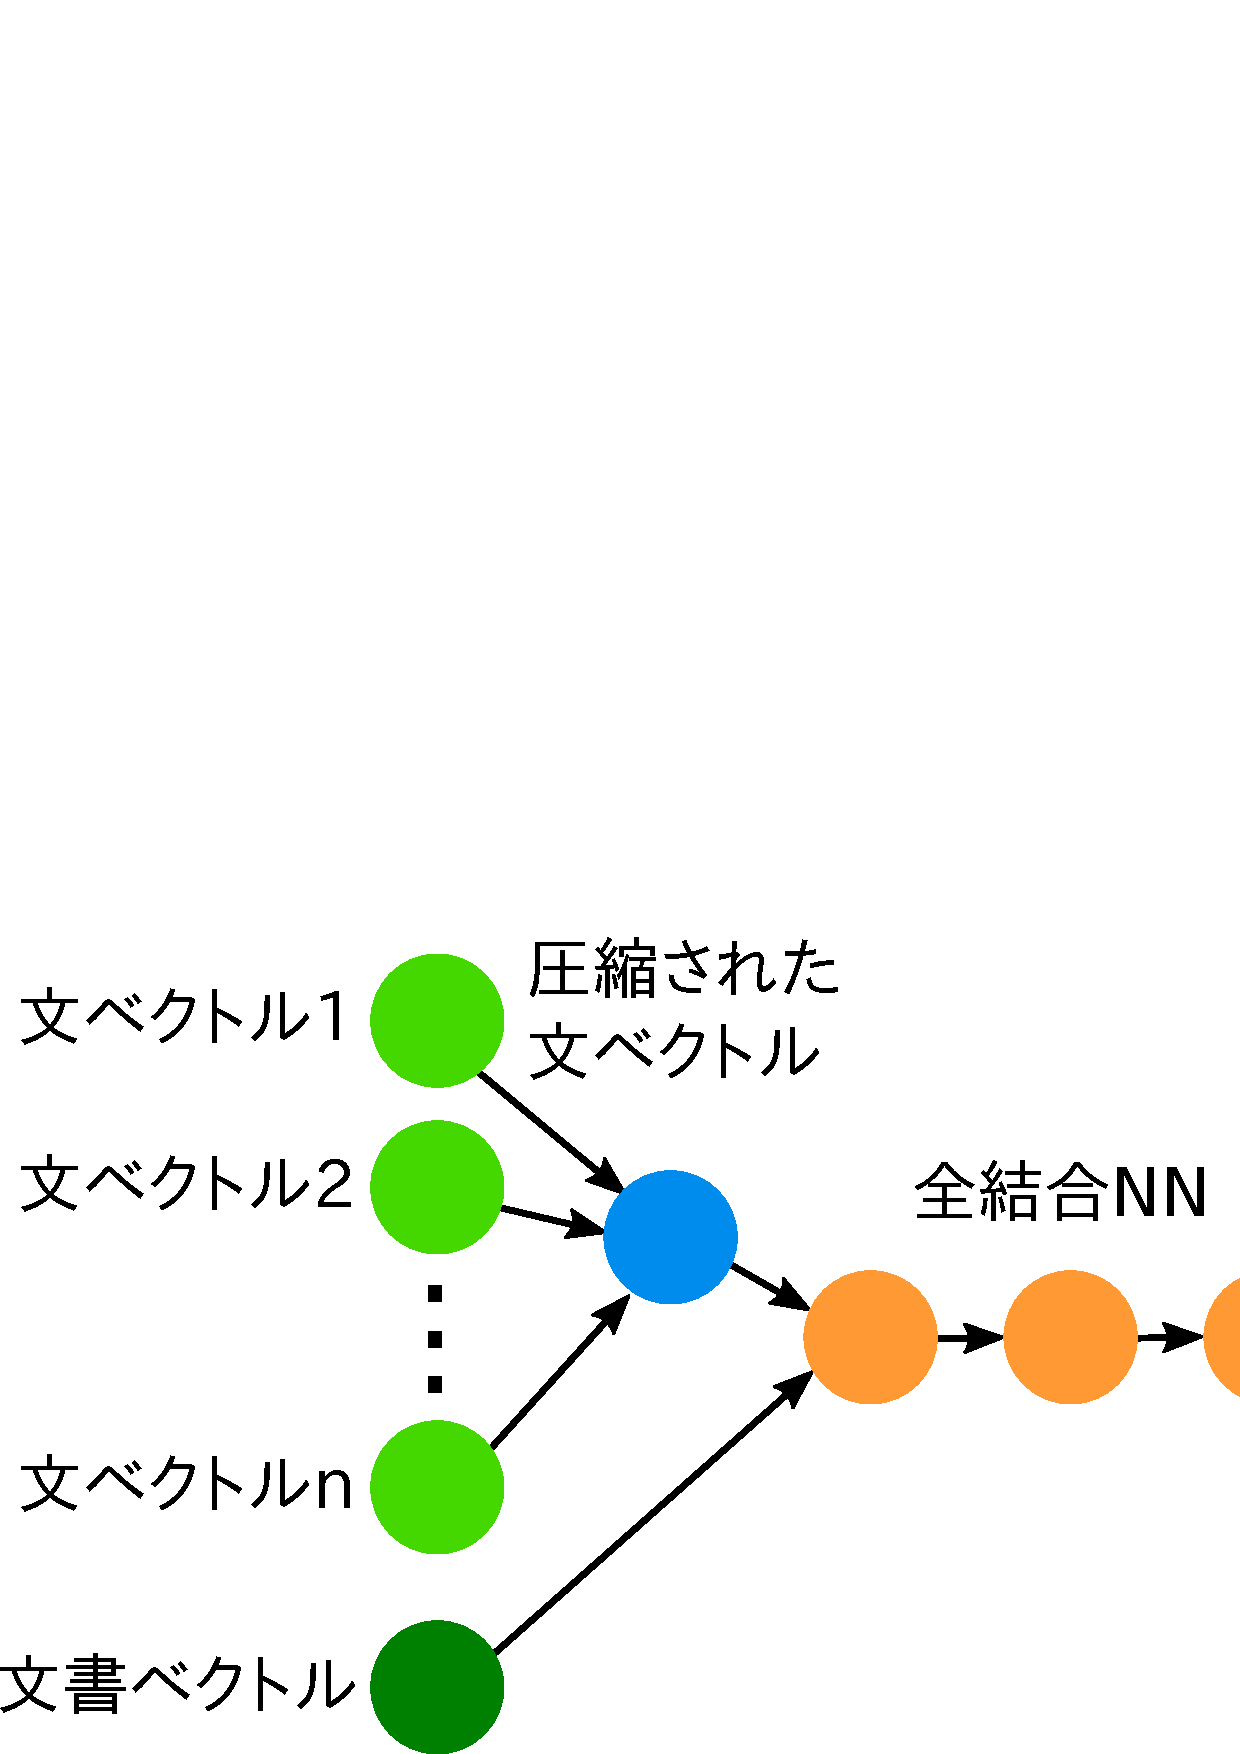
\includegraphics[width=\linewidth]{fig/model.png}}
  \end{textblock}
  \begin{block}{方法}
    \begin{itemize}
      \item \itemtitle{パラグラフベクトル}
        \begin{itemize}
          \item 文や文書を疎でない実数ベクトルに変換する手法
          \item 評判分類において優れる
        \end{itemize}
      \item \itemtitle{ニューラルネットワーク}
        \begin{itemize}
          \item 神経回路を模した機械学習手法
          \item 分類問題に用いることができる
          \item 文書・文間やカテゴリ間の複雑な関係を考慮できる
        \end{itemize}
    \end{itemize}
  \end{block}
\end{frame}

\begin{frame}{実験及び結果}{}
  \begin{block}{実験設定}
    \begin{itemize}
      \item
    \end{itemize}
  \end{block}
  \begin{block}{結果}
    \begin{itemize}
      \item
    \end{itemize}
  \end{block}
\end{frame}

\end{document}
